%% This is an example first chapter.  You should put chapter/appendix that you
%% write into a separate file, and add a line \include{yourfilename} to
%% main.tex, where `yourfilename.tex' is the name of the chapter/appendix file.
%% You can process specific files by typing their names in at the 
%% \files=
%% prompt when you run the file main.tex through LaTeX.
\chapter{Tujuan dan Manfaat Penelitian}
% Tujuan dan manfaat penelitian mencakup poin-poin yang diharapkan tercapai dari penelitian yang
% dilakukan, serta manfaat praktis yang diperoleh dari penelitian.

\section{Tujuan Penelitian}
% \\Gambar~\ref{fig:multipartite_graph} mengilustrasikan luaran dari sistem prediksi yang kami ajukan.

Tujuan dari penelitian ini adalah sebagai berikut:
\begin{enumerate} [topsep=0mm]
\itemsep0mm

\item
Mengembangkan metode prediksi yang akurat untuk estimasi interaksi antara senyawa bioaktif dengan protein.
Senyawa bioaktif tersebut berupa senyawa sintetis atau senyawa organik yang berasal baik dari tanaman-tanaman obat, 
sedangkan protein merupakan protein signifikan (biomarker) untuk suatu penyakit tertentu.
Kami berfokus pada metode-metode berbasis kernel (skor kesamaan).
Oleh karena itu, dua sub-tujuan yang mendukung adalah 
a)~perumusan kernel dan 
b)~pengembangan metode prediksi berbasis kernel (kernel-based machine learning).

\item
Membangun web-server yang handal untuk memberikan layanan publik mengenai prediksi interaksi antara senyawa bioaktif dengan protein.
Secara lugas, pengguna publik memasukkan, sebagai input, nama tanaman (atau senyawa bioaktif) dan nama penyakit (atau protein).
Selanjutnya, web-server akan melakukan prediksi interaksi keduanya dan menampilkan hasil prediksi beserta skor kepercayaannya dengan informatif.

\end{enumerate}

\begin{figure}[!b]
	\centering
	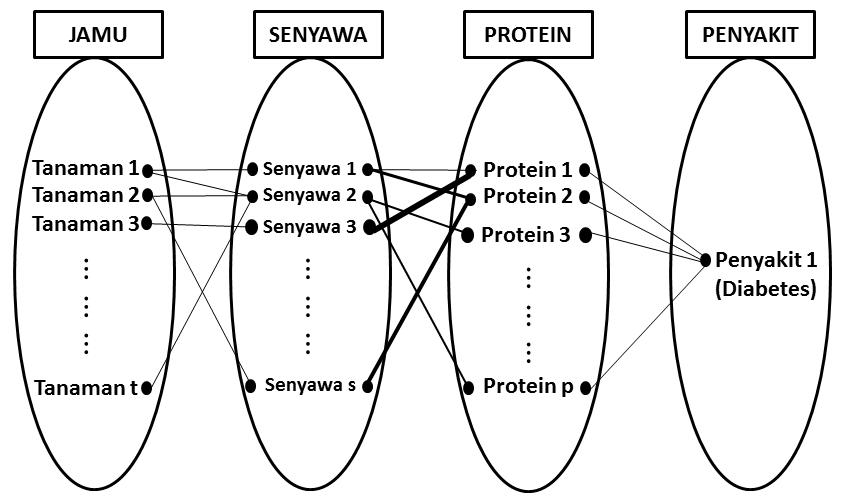
\includegraphics[height=0.45\linewidth]{multipartite-graph.png}
	\caption{Visualisasi \emph{multi-partite graph} hasil prediksi interaksi antara senyawa bioaktif tanaman obat dengan protein biomarker diabetes.
	Edge (garis konektifitas) antara himpunan senyawa dan protein memiliki bobot yang menunjukkan tingkat kepercayaan hasil prediksi; semakin terpercaya, maka bobot semakin besar (edge semakin tebal).
	Semakin banyak edge tebal antara himpunan senyawa dan protein, maka semakin besar pula potensi suatu Jamu menyembuhkan suatu penyakit.}
	\label{fig:multipartite_graph}
\end{figure}

\section{Manfaat Penelitian}
Manfaat dari penelitian ini adalah sebagai berikut:

\begin{enumerate} [topsep=0mm]
\itemsep0mm
\item
Prediksi yang akurat terhadap interaksi senyawa bioaktif dengan protein merupakan informasi yang krusial untuk pengembangan obat dan suplemen makanan, baik herbal maupun sintetis.
Dengan informasi ini sebagai penapis in-silico, uji klinis yang mahal dan lama hanya dilakukan pada kandidat senyawa yang berpotensi tinggi.

\item
Web-server publik yang handal berfungsi sebagai pusat informasi tentang (prediksi) khasiat tanaman obat.
Selain itu, kode web-server akan disediakan dalam bentuk open-source library dengan dokumentasi yang rapi dan lengkap sehingga dapat dimanfaatkan oleh peneliti.
Hal ini akan mendukung kesinambungan pengembangan dan perawatan sistem.
Kode tersebut meliputi fungsi-fungsi perhitungan kernel gabungan, proses prediksi, serta penjelajahan (crawling) database terkait.
\end{enumerate}
